\chapter{相关研究现状}

人机对话系统一直是人工智能领域的重要研究方向,其旨在模拟人类并与人类形成连贯通顺的对话。本文所研究的面向垂直领域的对话生成是对话系统领域的其中一个下游任务,因此本章先对管道式对话系统和端到端式对话系统的研究进展和现状进行总结。然后,分别介绍面向垂直领域的对话生成和基于大型语言模型的对话生成的发展现状,并分析和总结其优点与不足。

\section{对话系统}

近年来,深度学习技术快速发展,促进了对话系统研究的发展\cite{JSJX201907001}。目前主流的对话系统实现方法从架构模式来看,可以分为管道式对话系统和端到端式对话系统。

\subsection{管道式对话系统}

图\ref{pipeline_dialogue_system}展示了管道式对话系统(Pipeline-based Dialogue System)结构的示意图,管道式对话系统主要包含四个模块:(1)自然语言理解(NLU)模块;(2)对话状态跟踪(DST)模块;(3)对话策略学习(PL)模块;(4)自然语言生成(NLG)模块。

\begin{figure}[htbp]
	\centering
	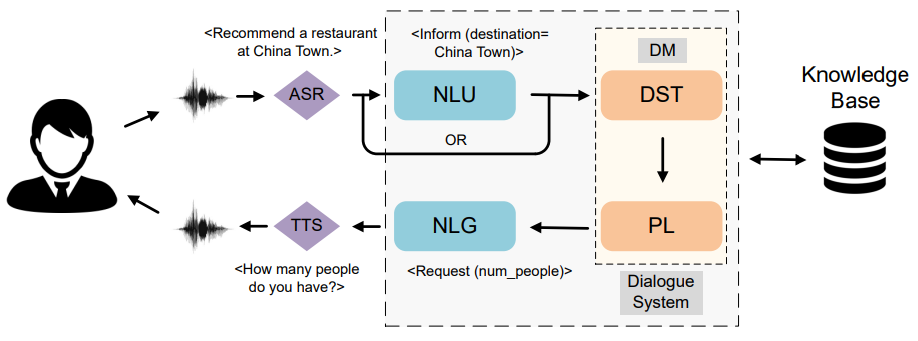
\includegraphics[scale=0.55]{Fig/pipeline_dialogue_system.png}
	\caption{\label{pipeline_dialogue_system}管道式对话系统结构示意图\cite{DBLP:journals/air/NiYPXC23}。}
\end{figure}

自然语言理解模块对原始的用户输入进行领域分类和意图识别,并提取其关键信息填入槽位中。
Deng等人\cite{DBLP:conf/slt/DengTHH12}和Tur等人\cite{DBLP:conf/icassp/TurDHH12}使用深凸网络将过去时间步的预测和当前消息结合起来,成功提高对话意图识别的准确率。
Sarikaya等人\cite{DBLP:journals/taslp/SarikayaHD14}使用受限玻尔兹曼机和深度置信网络初始化深度神经网络参数,解决了深度网络难以在领域分类和意图识别任务上训练的问题。
Ravuri等人\cite{DBLP:conf/interspeech/RavuriS15}利用循环神经网络(RNN)在序列预测上的优势,使用RNN对用户消息进行编码,以实现意图识别和领域分类。
Hashemi等人\cite{hashemi2016query}使用卷积神经网络(CNN)提取对话的多层级文本特征,以实现意图识别,同时该工作说明了CNN在序列预测任务上的可用性。
Lee等人\cite{DBLP:conf/naacl/LeeD16}使用RNN和CNN整合对话历史,获得上下文信息作为额外输入补充,解决了短语句信息不足的问题。
Wu等人\cite{DBLP:journals/corr/abs-2004-06871}提出预训练的面向任务对话BERT(TOD-BERT)模型提升意图识别任务上的准确率,同时所提出模型展现出小样本学习能力,缓解特定领域数据匮乏的问题。

对话状态跟踪模块根据当前用户消息和对话历史控制对话状态,以生成信息用于决定下一步动作。
Henderson等人\cite{DBLP:conf/sigdial/HendersonTY13}将深度学习模型用于对话状态跟踪,他们集成多种特征工程方法来预测每个槽-值对的概率。
Mrksic等人\cite{DBLP:conf/acl/MrksicSTGSVWY15}将RNN应用于对话状态跟踪以获得对话上下文感知。
随后,Mrksic等人\cite{DBLP:conf/acl/MrksicSWTY17}提出一种多跳的神经网络对话状态跟踪器,它使用系统输出、用户消息、候选槽值对作为输入,并基于对话历史对当前槽值对进行二分类预测。但是上述方法基于预定义的槽名与槽值,每一轮对话都需要对所有槽分别进行一次二分类,系统响应慢。
为了解决填槽类别多导致的计算复杂度高的问题,Lei等人\cite{DBLP:conf/acl/KanHLJRY18}提出信念片段,即一种与槽名相对应的对话上下文片段,通过构建一个两阶段CopyNet网络来拷贝和存储对话历史中的槽值,并用以生成回答,促进端到端训练,有效提升了系统在未登录词(OOV)下的准确度。
Wang等人\cite{DBLP:conf/emnlp/WangGZ20}提出了一种基于BERT模型的槽值预测方法,使用槽位注意力方法对相关片段进行检索,并使用槽值归一化方法将片段转化为最终的槽值。

对话策略学习模块根据对话状态决定下一步行为,主流方法是监督学习和强化学习。
Zhang等人\cite{DBLP:conf/acl/ZhangLGC19}提出一种高效资源调度方法,充分利用用户交互,在训练时使用概率调度器来分配对话样本,同时利用一个控制器决定使用真实样本还是模拟样本,有效提升强化学习训练的效果。
Takanobu等人\cite{DBLP:conf/acl/TakanobuLH20}提出一种多机对话策略学习方法,分别使用两个机器人扮演用户和系统,同时学习对话策略,同时,他们还加入特定角色的强化学习反馈,促进角色回答的生成。
Huang等人\cite{JSJX200408010}提出基于槽特征有限状态自动机的对话管理方法,通过树形的意图分层结构,实现多主题对话系统的主题检测与主题切换功能,并具有一定扩展性。

自然语言生成模块将系统的行为转化为自然语言,即最终输出,并返回给用户。
Wen等人\cite{DBLP:conf/sigdial/WenGKMSVY15}提出一种基于RNN的统计语言模型,通过语义约束和语法树学习回答生成,同时还使用CNN对候选回答进行排序,选出最佳回答。
Wen等人\cite{DBLP:conf/naacl/WenGMRSVY16}对循环语言模型采取先在大规模通用语料上预训练,然后在小规模特定领域语料上微调的训练方法,有效提升了循环语言模型的领域适应能力。
Li等人\cite{DBLP:conf/acl/LiYQCLL20}提出一种迭代矫正网络以迭代式修正所生成的标识符,首先使用监督学习训练网络,然后通过强化学习进行微调,并将槽位不一致的惩罚项添加到训练奖励中。

总结:管道式对话系统利用神经网络模型进行信息抽取和文本分类,而对话流程基于人工预定义的模板,因此特征相对固定,难以实现领域迁移。

\subsection{端到端式对话系统}

随着GPT\cite{DBLP:conf/nips/BrownMRSKDNSSAA20},BERT\cite{DBLP:conf/naacl/DevlinCLT19},T5\cite{DBLP:journals/jmlr/RaffelSRLNMZLL20}等序列到序列(Seq2Seq)\cite{DBLP:conf/nips/SutskeverVL14,DBLP:conf/emnlp/ChoMGBBSB14}预训练模型的兴起,基于Seq2Seq模型的端到端对话系统(End-to-End Dialogue System)逐渐成为主流。这类方法将对话系统的核心功能隐式地集成到一个复杂的神经网络模型当中,降低了系统模块复杂度。从研究侧重点上来看,端到端式对话系统的研究可分为两类:(1)基于模型架构的研究;(2)基于训练方法的研究。

Sordoni等人\cite{DBLP:conf/cikm/SordoniBVLSN15}提出一种上下文感知的Seq2Seq模型HRED,该模型同时学习字符级和对话级的文本表示,有效解决上下文感知的在线查询建议问题,提供少见且高质量的结果。
Serban等人\cite{DBLP:conf/aaai/SerbanSLCPCB17}进一步提出VHRED模型,对序列间的复杂依赖进行建模,通过在解码器中增加一个隐变量,在回答的多样性、长度和质量上都有一定的提升。
Weston等人\cite{DBLP:journals/corr/WestonCB14}提出一种记忆网络,使用RNN网络在每个时间步上向后传递历史信息。然而,这种模型包含五个模块,每个模块都需要单独进行监督训练,因此不适用于端到端式对话系统。
Sukhbaatar等人\cite{DBLP:conf/nips/SukhbaatarSWF15}在他们的工作基础上,提出了一种端到端的记忆网络,引入注意力方法,依次进行权重计算、记忆选择、最终预测。
在某些对话场景下,对话系统需要直接从用户输入中引用或摘要内容,而传统Seq2Seq模型的输出维度受限于输入的维度。
为解决该问题,Oriol等人\cite{DBLP:conf/nips/VinyalsFJ15}提出Pointer Net,每个时间步的输出都来自输入序列,将标识符预测问题转化为位置预测问题,以适应输入长度的变化。
然而,Pointer Net仅从输入中选择标识符的局限性较大,Gu等人\cite{DBLP:conf/acl/GuLLL16}提出CopyNet,在解码阶段的每个时间步中,决定复制输入中的标识符还是生成一个新的标识符,将复制概率和生成概率加和,得到最终的预测概率。
Balakrishnan等人\cite{DBLP:conf/acl/BalakrishnanRUW19}提出一种约束解码模块,以提升对话系统所生成回答的语义准确性。
Chen等人\cite{DBLP:conf/acl/ChenXX19}使用两个长期记忆模块分别存储知识元组和对话历史,然后用一个工作记忆模块来控制标识符的生成,有效提升对话相关知识的检索精确度。
Gao等人\cite{DBLP:conf/acl/GaoZOY20}使用一个释义模型对回答生成模型进行增强,释义模型与整个对话系统联合训练,用于增强训练样本。

Wang等人\cite{DBLP:conf/acl/WangZLHZL19}提出一种基于增量学习的训练方法,通过构建一个不确定性估计模块,在模型所生成回复的自信度低于阈值时使用人类回答作为结果,同时通过在线学习拟合人类回答,有效提升了模型回复质量。
Dai等人\cite{DBLP:conf/acl/DaiLTLSZ20}使用模型无关的元学习方法,仅依靠少量训练样本,在真实线上服务场景下有效提升模型的迁移能力和可靠性。
He等人\cite{DBLP:conf/emnlp/HeYYLSX20}提出一种“双教师单学生”知识蒸馏训练框架,首先两个教师模型分别以知识检索和回答生成作为训练目标,进行强化学习训练,然后让学生模型模仿教师模型的输出,实现专业知识的迁移。
Zhang等人\cite{DBLP:conf/acl/ZhangSGCBGGLD20}使用GPT-2\cite{radford2019language}作为基座模型,在Reddit社交媒体语料上训练,并引入最大互信息(MMI)评分函数,使对话系统能生成更相关、内容丰富、上下文一致的回复。
Daniel等人\cite{DBLP:journals/corr/abs-2001-09977}提出基于Evolved Transformer的Meena架构模型,将模型参数量扩充至2.6B,同时提出对话评估指标SSA,包含逻辑性和特异性两个维度,适用于对话模型的大规模人工评估场景,具有易于理解、一致性高等优势。
Roller等人\cite{DBLP:conf/eacl/RollerDGJWLXOSB21}使用具有特定对话能力的BST数据集对预训练模型进行微调,得到BlenderBot模型,BST数据集涵盖引人入胜、善于倾听、博学、同理心、有个性等对话能力,同时对比了检索式、生成式、混合式三种基于Transformer的模型架构,最终生成式模型的表现超过当时的最先进方法。
Bao等人\cite{DBLP:conf/acl/BaoHWWW20}提出对话行为隐变量,用以表征不同的说话风格,进而生成多样的回答,使用该方法在对话语料上训练BERT得到PLATO模型,该模型具备多轮流畅对话能力。

总结:端到端式对话系统的架构相对简单,且生成的回复更多样。然而,这类对话系统通常需要大量高质量对话语料,且模型尺寸一般比较大,训练资源开销大。

\section{面向垂直领域的对话生成}

垂直领域的对话内容相较于开放域对话具有更强的知识性与复杂性,直接使用开放域对话生成的方法无法得到准确可靠的回复。为此,许多研究者对面向垂直领域的对话生成展开研究。面向垂直领域的对话生成方法主要分为两类:(1)基于外部知识的方法;(2)基于知识注入的方法。

\subsection{基于外部知识的垂直领域对话生成}

Lin等人\cite{DBLP:conf/acl/LinJHWC20}提出基于拷贝机制的知识对话方法KIC,将循环知识交互解码器与知识感知的Pointer Net相结合,实现知识生成和知识拷贝。
Wu等人\cite{DBLP:conf/acl/WuLZZW20}采用一个多类别分类器对生成的单词、生成的知识实体和拷贝的查询单词进行融合,提升了模型生成回答的准确性、一致性和知识性。
Majumder等人\cite{DBLP:conf/emnlp/MajumderJBM20}同时进行角色信息选择和基于角色的响应生成,并使用强化学习训练对话智能体。
Moon等人\cite{DBLP:conf/acl/MoonSKS19}结合知识图谱与对话系统,将知识图谱信息作为外部知识,在强化学习框架中,智能体基于当前节点和状态选择相应的边,然后将知识组合到回答生成过程中。
Xu等人\cite{DBLP:conf/acl/XuWNWCL20}将知识图谱作为外部知识,控制粗粒度的对话生成,对话具有常识性知识支撑,使得智能体能更好地引导对话话题。
Jung等人\cite{DBLP:conf/emnlp/JungSL20}提出双向图探索模型AttnIO,用于在结构化知识图谱中检索外部知识,通过在遍历的每一步中计算注意力权重,使得模型能够选择更大范围的知识路径。
Yang等人\cite{DBLP:conf/emnlp/YangZE20}提出基于知识图谱的对话方法GraphDialog,首先将对话历史解析为依赖关系树,并编码为嵌入向量,然后使用注意力机制对知识图谱进行多跳推理,最后由解码器从图谱中拷贝实体或预测单词,实现将垂直领域知识图谱中的外部知识整合到模型回复中。
Lv等人\cite{SJSJ202312037}提出嵌入知识语义的医疗领域对话系统,使用BERT融合BiLSTM的对话训练方法,将医疗知识图谱的语义信息融入对话系统。

总结:基于外部知识的垂直领域对话生成方法主要基于符号逻辑或知识图谱来实现外部知识的补充。然而,这类方法无法有效建模未见过的实体,且没有考虑互联网上大量的文本信息,导致泛化性和实时性不足。

\subsection{基于知识注入的垂直领域对话生成}

Wu等人\cite{DBLP:journals/corr/abs-2303-17564}提出BloombergGPT金融大模型,使用通用语料与金融领域语料混合的数据集,从头训练领域大模型,在模型学习基本语言语法和世界常识的同时,注入垂直领域知识。然而,从头开始预训练大模型需要收集大规模的通用语料,同时提高模型后续在语言层面的迁移难度。因此,较为主流的知识注入方式是在预训练通用模型的基础上进行继续预训练或监督微调。
Zhang等人\cite{DBLP:conf/cikm/ZhangY23}提出XuanYuan金融领域大模型在预训练语言模型Bloom的基础上使用混合数据继续预训练,混合数据包含通用领域数据和金融领域内的专业知识数据,并采用Hybrid-Tuning训练策略,在提升模型领域内能力的基础上,保证模型通用能力不会退化。
Meng等人\cite{DBLP:conf/sigir/MengRCSRTR20}提出DukeNet,构建了一个双向知识交互网络,实现面向垂直领域知识的对话生成。
Chen等人\cite{DBLP:journals/corr/abs-2310-15896}提出扁鹊模型,通过构建高质量的医学领域对话数据集,得到预训练模型在下游对话任务上的良好性能。
Zhou等人\cite{DBLP:conf/acl/ZhouZHHZ20}提出KdConv,即中文多领域知识驱动对话数据集,通过在数据集上训练将知识注入模型中。
上述方法都需要构建大规模高质量领域内训练语料,对于垂直领域对话生成任务,往往还需要耗费人力,将其处理为“指令-回答”格式的对话数据,因此高质量的领域对话数据集十分稀缺。为解决数据稀缺的问题,Wang等人\cite{DBLP:conf/acl/WangKMLSKH23}提出Self-Instruct方法,利用大型语言模型对小规模的种子样本进行数据扩充,以生成更多符合要求的微调数据。
Zhang等人\cite{DBLP:journals/corr/abs-2305-11952}提出Self-QA方法,直接基于非结构化文档数据生成指令数据,无需初始种子数据,进一步降低了数据扩充的人力成本。
Wang等人\cite{DBLP:journals/corr/abs-2304-06975}提出Self-KG方法,基于中文医药知识图谱CMeKG生成指令数据,利用知识图谱中的节点关联信息,生成更高质量的指令数据。

总结:基于知识注入的垂直领域对话生成方法需要收集大规模高质量对话语料用于训练,同时知识被隐式存储在模型参数中,难以及时更新。

\section{基于大型语言模型的对话生成}

近年来,随着ChatGPT\cite{DBLP:conf/nips/Ouyang0JAWMZASR22}的发布,国内外先后出现许多预训练大型语言模型,如ChatGLM\cite{DBLP:conf/iclr/ZengLDWL0YXZXTM23}、文心一言\cite{DBLP:journals/corr/abs-2107-02137}、通义千问\cite{DBLP:journals/corr/abs-2309-16609}、LLaMA\cite{DBLP:journals/corr/abs-2302-13971}、百川\cite{DBLP:journals/corr/abs-2309-10305}等。因此,越来越多的研究者将大型语言模型作为对话生成研究的基础。
基于大型语言模型的对话生成可分为两类:(1)基于提示词工程的方法;(2)基于监督数据微调的方法。

\subsection{基于提示工程的对话生成}

Radford等人\cite{radford2019language}提出Zero-shot提示方法,利用大型语言模型进行范式迁移,无需训练即可让预训练模型完成下游任务,但该方法得到的输出可能不够准确或不符合预期。
为此,Brown等人\cite{DBLP:conf/nips/BrownMRSKDNSSAA20}提出Few-shot提示方法,在模型输入中提供高质量的示例,提升模型在复杂任务上的性能。
Wei等人\cite{DBLP:conf/nips/Wei0SBIXCLZ22}提出思维链(Chain-of-Thought,CoT)提示方法,通过在模型输入的结尾引导模型一步步思考,并在给出回复前先对问题进行拆解和分析,使得模型最终输出的答案更加准确。
Wang等人\cite{DBLP:conf/iclr/0002WSLCNCZ23}引入自洽性(Self-Consistency)解码策略,通过采样生成多条推理链,然后采用投票方法从这些推理链中选出一致性最高的答案,在GSM8K复杂推理数据集上,Self-Consistency相比于CoT方法有17.9\%的提升,证明该方法能很好的提升LLM的复杂任务推理能力。
Long等人\cite{DBLP:journals/corr/abs-2305-08291}提出思维树(Tree-of-Thought,ToT)提示方法,ToT是对CoT方法的扩展,通过管理树结构的中间推理步骤,同时使用深度优先或广度优先等搜索算法,对推理链路进行系统性扩展,使模型在得到错误答案时能够进行回溯,ToT在24类游戏任务上取得了74\%的成功率,而CoT仅有4\%。
Yao等人\cite{DBLP:journals/corr/abs-2305-16582}提出思维图(Graph-of-Thought,GoT)提示方法,使用基于图的架构,更好地适应人类非线性思考地特性。这类方法不需要重新训练模型即可提升模型性能,但提升受限于预训练模型自身的能力上限。

总结:提示工程方法的复杂度和成本相对较低,具有较高的灵活性,但生成的结果准确性受限于基座模型自身的能力,通常会出现不符合事实的回答,难以应对垂直领域对话。

\subsection{基于检索增强的对话生成}

大型语言模型具有良好的自然语言理解和自然语言生成能力,但往往面临幻觉问题,即回复内容不符合事实,甚至胡编乱造。这可能是因为模型在预训练阶段记忆了错误的知识,或是推理时的输入是预训练阶段没有遇到过的长尾知识。
针对后者,Lewis等人\cite{DBLP:conf/nips/LewisPPPKGKLYR020}提出检索增强生成(Retrieval Augmented Generation,RAG)技术,通过构建本地知识库,在对话阶段从知识库中召回与用户问题相关的文档,作为外部知识辅助语言模型给出回复,很好地缓解了大型语言模型的幻觉问题和实时性不足的问题。
Wang等人\cite{DBLP:conf/emnlp/WangYW23}提出Query2doc方法,利用大型语言模型对用户问题生成伪文档,以提升知识库的召回准确度,以减少无关文档对语言模型回复产生噪声干扰。
Jagerman等人\cite{DBLP:journals/corr/abs-2305-03653}在Query2doc方法的基础上提出思维链技术与伪相关反馈(Pseudo-Relevance Feedback,PRF)算法相结合的方法,在多个基准数据集上获得了超过Query2doc方法的效果。
Liu等人\cite{DBLP:journals/corr/abs-2307-03172}的研究表明,当相关信息出现在模型输入上下文的开头或结尾时,模型的性能最好,相关信息出现在中间位置时模型表现最差,且随着输入上下文的增长,模型性能显著下降,表明模型很难从长输入上下文中检索和使用相关信息。因此召回的知识文档数量及其在模型输入中的位置对模型性能至关重要。
Asai等人\cite{DBLP:journals/corr/abs-2310-11511}提出Self-RAG方法,生成模型通过检索召回多个相关文档,并通过并行处理和排序选择最合适的回复。
Cui等人\cite{DBLP:journals/corr/abs-2306-16092}提出ChatLaw中文法律大模型,在RAG的基础上。融入法律意图识别、法律关键词提取等模块,满足法律相关领域的应用需求。这类方法在背景知识丰富且逻辑相对复杂的专业领域上表现不佳。

总结:检索增强方法能很好地改善大型语言模型的幻觉问题,得到高准确性的回复。然而,现有的检索增强方法更多的关注如何提升外部知识的召回准确性,没有考虑基座模型内部知识与外部知识之间的偏差,存在性能瓶颈。

\subsection{基于模型微调的对话生成}

Wei等人\cite{DBLP:conf/iclr/WeiBZGYLDDL22}提出指令微调(Instruction Tuning)方法,通过监督训练,让语言模型学会按照指令要求完成任务,从而具备遵循指令的能力,即使面对训练中未曾见过的任务,模型也能够生成合适的回复。
Li等人\cite{DBLP:conf/acl/LiL20}提出Prefix-Tuning方法,在模型输入首端增加一个连续的、任务相关的嵌入向量来进行训练,在显著减少训练参数量的情况下提升模型在自然语言生成任务上的性能。
与Prefix-Tuning思想相似,Brian等人\cite{lester-etal-2021-power}提出提示学习(Prompt Tuning)方法,通过在输入中插入一段任务特定的、可被训练的离散提示词元,获得了与微调相近的效果,同时超过了人工设计提示词的性能。
Liu等人\cite{DBLP:journals/corr/abs-2110-07602}在Prefix-Tuning的基础上,进一步提出P-Tuning v2方法,在模型的每一层上都加上了可训练的层级提示词元,且对于不同难度的任务使用不同的提示长度。
Hu等人\cite{DBLP:conf/iclr/HuSWALWWC22}提出了低秩自适应(Low-Rank Adaptation,LoRA)方法,通过使用低维结构来近似大模型的高维结构,以降低模型训练的复杂度和计算开销。总体来说,基于监督数据微调的方法性能优于基于提示词工程的方法,但存在高质量标注数据难获取的问题。

Long等人\cite{DBLP:conf/nips/Ouyang0JAWMZASR22}提出基于人类反馈的强化学习(Reinforcement Learning with Human Feedback,RLHF)算法,其工作过程包括采集高质量数据集对语言模型监督微调(SFT)、收集人类偏好排名数据集并训练奖励模型(RM)、执行近端策略优化(Proximal Policy Optimization,PPO)强化学习。
该算法能够很好地帮助模型生成符合人类偏好的回复,同时减少生成式模型中的偏见。然而,RLHF算法在PPO强化学习训练阶段需要同时使用四个大型语言模型,导致训练计算资源开销大,同时PPO强化学习过程不稳定,导致模型难以训练。为此,许多研究者提出其他的人类偏好对齐算法替代RLHF算法。
Li等人\cite{DBLP:journals/corr/abs-2309-07124}提出RAIN可回滚自回归推理算法,利用语言模型评估自己生成的结果,并用评估结果来指导语言模型输出,以确保输出符合人类偏好,无需微调即可实现语言模型与人类偏好的对齐。
Zheng等人\cite{DBLP:journals/corr/abs-2307-04964}针对PPO训练不稳定的问题,通过实验探索了PPO训练中最关键的技巧,并用PPO-max表示这套最佳实现方式。
Dong等人\cite{DBLP:journals/corr/abs-2304-06767}提出RAFT方法,在采集的人类偏好数据中选取多个高质量样本,继续对SFT模型进行监督微调,利用更多次采样和更少的梯度计算,让模型更稳定和鲁棒。
Yuan等人\cite{DBLP:journals/corr/abs-2304-05302}在RLHF的基础上提出RRHF算法,直接使用偏好数据训练语言模型,结合排名损失和SFT损失,在性能上与PPO方法相近,但实现相对简单且训练稳定。
Cheng等人\cite{DBLP:journals/corr/abs-2311-04155}提出BPO黑盒提示优化算法,通过采集人类偏好数据,训练提示优化器,对用户指令进行优化,使模型生成的内容更符合用户期望。
Rafailov等人\cite{DBLP:conf/nips/RafailovSMMEF23}提出DPO算法,其思想与RRHF相似,但同时引入SFT模型的约束,保证在不使用SFT损失的情况下训练依然稳定,该方法在多个开源RM数据集上获得优于RLHF的奖励得分,且对超参数的敏感度更低,效果更稳定。
Liu等人\cite{DBLP:journals/corr/abs-2309-06657}提出RSO算法,使用拒绝采样得到高质量回答的分布。
上述方法依赖于人类反馈数据,标注成本高昂。为解决该问题,Bai等人\cite{DBLP:journals/corr/abs-2212-08073}提出RLAIF方法,用宪法人工智能(CAI)代替人类进行偏好的标记工作,实验表明RLAIF能够达到与RLHF相当的性能。
此外,Li等人\cite{DBLP:journals/corr/abs-2310-10505}提出ReMax算法,通过削减PPO中冗余庞大的计算开销,节省RLHF算法50\%的内存消耗,并加快2倍训练速度。现有方法一方面需要高昂的人力成本完成偏好数据标注,另一方面存在训练计算资源开销大、难训练的问题。

总结:模型微调方法通过调整模型内部参数,能够控制模型内在的行为模式,对齐人类偏好,但是对动态数据缺乏实时性,难以及时跟进垂直领域的新知识。

\section{本章小结}

本章主要对研究相关的对话系统、面向垂直领域的对话生成以及基于大型语言模型的对话生成进行了介绍。总体而言,本章先介绍了对话系统在管道式对话系统和端到端式对话系统等方向的相关进展。然后,本章介绍了基于外部知识和基于知识注入的垂直领域对话生成方法的研究进展。最后,本章对基于大型语言模型的对话生成任务在基于提示工程、基于检索增强和基于模型微调方法的研究现状作了相关概述。